% Here we usae providecommand in case of Combinatorial_map.tex was used before
% this file.
\providecommand{\nulldart}{\ccc{null\_dart\_handle}}

\providecommand{\betats}{\ccTexHtml{$\beta$}{&beta;}}
\providecommand{\betazero}{\ccTexHtml{$\beta_0$}{&beta;<SUB>0</SUB>}}
\providecommand{\betaun}{\ccTexHtml{$\beta_1$}{&beta;<SUB>1</SUB>}}
\providecommand{\betadeux}{\ccTexHtml{$\beta_2$}{&beta;<SUB>2</SUB>}}
\providecommand{\betatrois}{\ccTexHtml{$\beta_3$}{&beta;<SUB>3</SUB>}}
\providecommand{\betaquatre}{\ccTexHtml{$\beta_4$}{&beta;<SUB>4</SUB>}}
\providecommand{\betai}{\ccTexHtml{$\beta_i$}{&beta;<SUB>i</SUB>}}
\providecommand{\betad}{\ccTexHtml{$\beta_d$}{&beta;<SUB>d</SUB>}}	
\providecommand{\betadprim}{\ccTexHtml{$\beta_{d'}$}{&beta;<SUB>d'</SUB>}}
\providecommand{\betaimun}{\ccTexHtml{$\beta_{i-1}$}{&beta;<SUB>i-1</SUB>}}
\providecommand{\betaipun}{\ccTexHtml{$\beta_{i+1}$}{&beta;<SUB>i+1</SUB>}}
\providecommand{\betaimdeux}{\ccTexHtml{$\beta_{i-2}$}{&beta;<SUB>i-2</SUB>}}
\providecommand{\betaipdeux}{\ccTexHtml{$\beta_{i+2}$}{&beta;<SUB>i+2</SUB>}}
\providecommand{\betaj}{\ccTexHtml{$\beta_j$}{&beta;<SUB>j</SUB>}}
\providecommand{\betajmun}{\ccTexHtml{$\beta_{j-1}$}{&beta;<SUB>j-1</SUB>}}
\providecommand{\betaiinv}{\ccTexHtml{$\beta_i^{-1}$}{&beta;<sub>i</sub><sup>-1</sup>}}
\providecommand{\betajinv}{\ccTexHtml{$\beta_j^{-1}$}{&beta;<sub>j</sub><sup>-1</sup>}}

\providecommand{\comp}{\ccTexHtml{$\circ$}{&deg;}}
\providecommand{\pinv}{\ccTexHtml{$p^{-1}$}{p<SUP>-1</SUP>}}
\providecommand{\myith}{\ccTexHtml{$i^{\mbox{th}}$}{i<SUP>th</SUP>}}

\providecommand{\myneq}{\ccTexHtml{$\neq$}{&ne;}}
\providecommand{\myleq}{\ccTexHtml{$\leq$}{&le;}}
\providecommand{\mylt}{\ccTexHtml{$<$}{&lt;}}
\providecommand{\mygt}{\ccTexHtml{$>$}{&gt;}}
\providecommand{\mygeq}{\ccTexHtml{$\geq$}{&ge;}}
\providecommand{\mysubseteq}{\ccTexHtml{$\subseteq$}{&sube;}}
\providecommand{\myforall}{\ccTexHtml{$\forall$}{&forall;}}
\providecommand{\myemptyset}{\ccTexHtml{$\emptyset$}{&empty;}}
\providecommand{\myRightarrow}{\ccTexHtml{$\Rightarrow$}{&rArr;}}
\providecommand{\myrightarrow}{\ccTexHtml{$\rightarrow$}{&rarr;}}
\providecommand{\myin}{\ccTexHtml{$\in$}{&isin;}}
\providecommand{\mynotin}{\ccTexHtml{$\notin$}{&notin;}}
\providecommand{\mycup}{\ccTexHtml{$\cup$}{&cup;}}
\providecommand{\myphi}{\ccTexHtml{$\phi$}{&phi;}}
\providecommand{\mysetminus}{\ccTexHtml{$\setminus$}{\ }}
\providecommand{\myldots}{\ccTexHtml{$\ldots$}{&hellip;}}
\providecommand{\mytimes}{\ccTexHtml{$\times$}{&times;}}

\providecommand{\cell}[1]{\emph{#1}-cell}
\providecommand{\cells}[1]{\emph{#1}-cells}
\providecommand{\orbit}[1]{\ccTexHtml{$\langle{}$}{&lang;}#1\ccTexHtml{$\rangle{}$}{&rang;}}




\section{Introduction}

A \emph{d}D linear cell complex allows to represent an orientable
subdivided \emph{d}D object having linear geometry: each vertex of the
subdivision is associated with a point. The geometry of each edge is a
segment whose end points are associated with the two vertices of the
edge, the geometry of each 2-cell is obtained from all the segments
associated to the edges describing the boundary of the 2-cell and so
on.

The combinatorial part of a linear cell complex is described by a
\emph{d}D combinatorial map (it is strongly recommended to first
read \ccRef[the combinatorial maps chapter]{ChapterCombinatorialMap}
for definitions).  To add
the linear geometrical embedding, a point (a model of
\ccc{CGAL::Point_2} or \ccc{CGAL::Point_3} or \ccc{CGAL::Point_d}) is
associated to each vertex of the combinatorial map.

%%%%%%%%%%%%%%%%%%%%%%%%%%%%%%%%%%%%%%%%%
\begin{figure}[ht]
  \begin{ccTexOnly}
    \begin{center}
      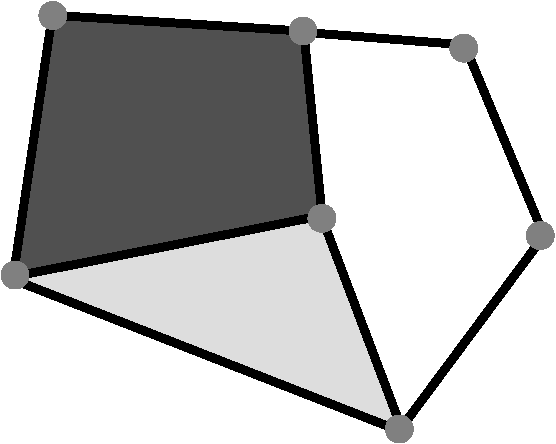
\includegraphics[width=.35\textwidth]
      {Linear_cell_complex/fig/pdf/object2d}
      \qquad
      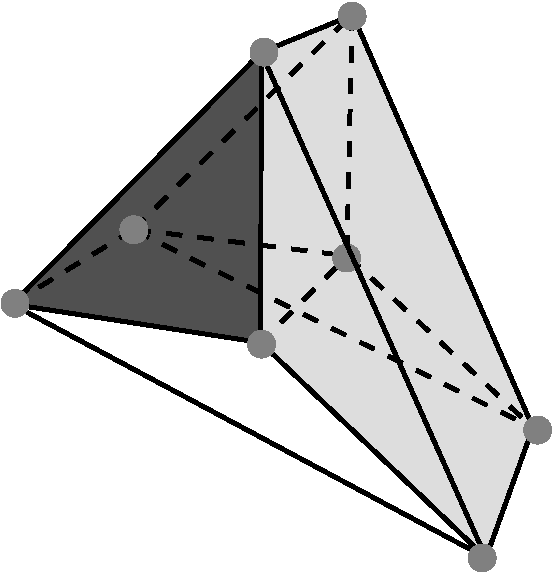
\includegraphics[width=.45\textwidth]
      {Linear_cell_complex/fig/pdf/intuitif-example-lcc-object}
    \end{center}
  \end{ccTexOnly}
  \begin{ccHtmlOnly}
    <CENTER>
    <A HREF="fig/png/object2d.png"><img src="fig/png/object2d.png" alt=""></A>
    <A HREF="fig/png/intuitif-example-lcc-object.png"><img src="fig/png/intuitif-example-lcc-object.png" alt=""></A>
    </CENTER>
    \end{ccHtmlOnly}
    \caption{Examples of objects with linear geometry. \textbf{Left}:~A
      2D object composed of three 2-cells, nine
      1-cells and seven points associated to the seven 0-cells .   
      \textbf{Right}:~A
      3D object composed of three 3-cells, twelve 2-cells, sixteen
      1-cells and eight points associated to the eight 0-cells.
      \label{fig-exemple-introductif}}
\end{figure}
%
If we reconsider the example introduced in the combinatorial map
package, recalled in Figure~\ref{fig-exemple-introductif} (Right), the
combinatorial part of the 3D object is described by a 3D combinatorial
map. As illustrated in Figure~\ref{fig-exemple-introductif-lcc}, the
geometrical part of the object is described by associating a point to
each vertex of the map.
%
\def\LargFig{.3\textwidth}
\begin{figure}[h]
  \begin{ccTexOnly}
    \begin{center}
      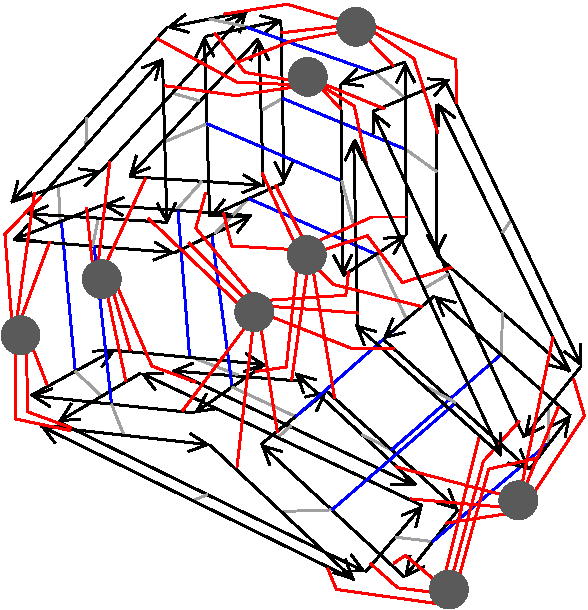
\includegraphics[width=\LargFig]{Linear_cell_complex/fig/pdf/intuitif-example-lcc}\qquad
      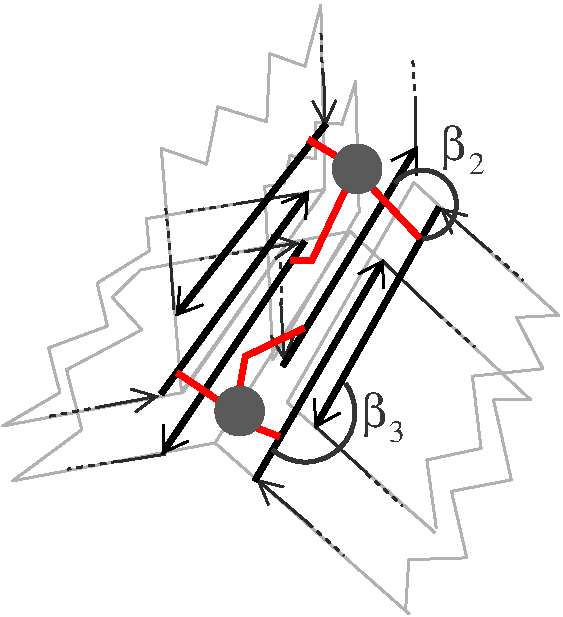
\includegraphics[width=\LargFig]{Linear_cell_complex/fig/pdf/intuitif-example-lcc-zoom}
      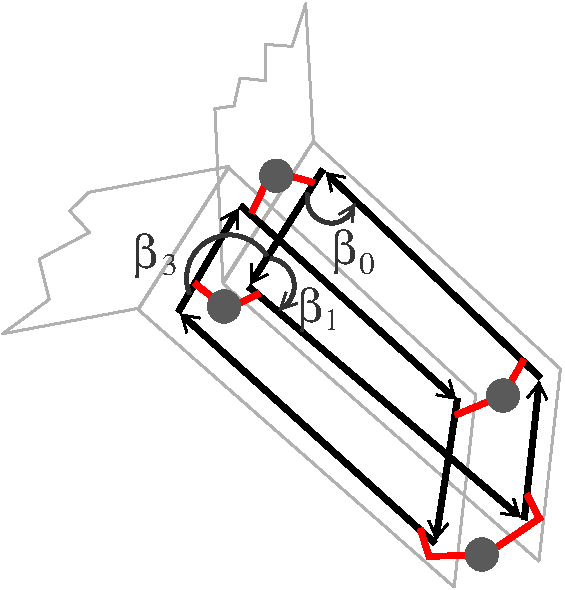
\includegraphics[width=\LargFig]{Linear_cell_complex/fig/pdf/intuitif-example-lcc-zoom2}
    \end{center}
  \end{ccTexOnly}
  \begin{ccHtmlOnly}
    <CENTER>
    <A HREF="fig/png/intuitif-example-lcc.png">
    <img src="fig/png/intuitif-example-lcc.png" alt=""></A>
    <A HREF="fig/png/intuitif-example-lcc-zoom.png">
        <img src="fig/png/intuitif-example-lcc-zoom.png" alt=""></A>
    <A HREF="fig/png/intuitif-example-lcc-zoom2.png">
        <img src="fig/png/intuitif-example-lcc-zoom2.png" alt=""></A>
    </CENTER>
    \end{ccHtmlOnly}
    \caption{Example of 3D linear cell complex describing the object
      given in Figure~\ref{fig-exemple-introductif} (Right).
      \textbf{Left}:~The 3D linear cell complex which contains 54 darts
      (18 for each 3-cell) where each vertex is associated with a
      point, here a \ccc{CGAL::Point_3}. Blue segments represent \betatrois{} relations.
      \textbf{Middle}:~Zoom around
      the central edge which details the six darts belonging to the
      edge and the associations between darts and points.
      \textbf{Right}:~Zoom around the facet between light gray and
      white 3-cells, which details the eight darts belonging to the
      facet and the associations between darts and
      points (given by red segments).\label{fig-exemple-introductif-lcc}}
\end{figure}

Note that the dimension of the combinatorial map \emph{d} is not
necessarily equal to the dimension of the ambient space
\emph{d2}. Indeed, we can use for example a 2D combinatorial map in a
2D ambient space to describe a planar graph
(\emph{d}=\emph{d2}=\emph{2}), or a 2D combinatorial map in a 3D
ambient space to describe a surface in 3D space (\emph{d}=2,
\emph{d2}=3) (case of the \ccc{Polyhedron_3} package), or a 3D
combinatorial map in a 3D ambient space (\emph{d}=\emph{d2}=3) and so
on.

\section{Software Design}

The diagram in Figure~\ref{fig-diagram_class_lcc} shows the main
classes of the package.  \ccc{CGAL::Linear_cell_complex} is the main
class (see Section~\ref{ssec-linear-cell-complex}), which inherits from
the \ccc{CGAL::Combinatorial_map} class.  Attributes can be associated
to some cells of the linear cell complex thanks to an items class (see
Section~\ref{ssec-lcc-item}), which defines the dart type and the
attributes types. These types may be different for different
dimensions of cells, and they may also be void.  In the class
\ccc{CGAL::Linear_cell_complex}, it is required that
specific attributes are associated to all vertices of the
combinatorial map. These attributes must contain a point (a model of
\ccc{CGAL::Point_2} or \ccc{CGAL::Point_3} or \ccc{CGAL::Point_d}),
and can be represented by instances of class
\ccc{CGAL::Cell_attribute_with_point} (see
Section~\ref{ssec-attribute-wp}).
%
\begin{figure}
  \begin{ccTexOnly}
    \begin{center}
      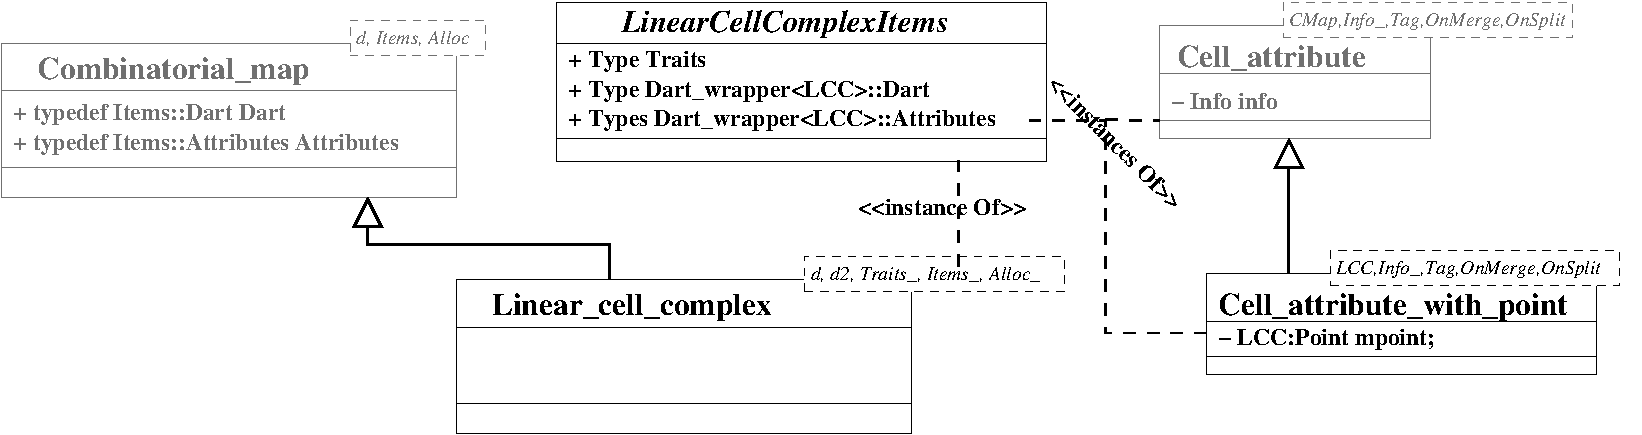
\includegraphics[width=.95\textwidth]
      {Linear_cell_complex/fig/pdf/Diagramme_class}
    \end{center}
  \end{ccTexOnly}
  \begin{ccHtmlOnly}
    <CENTER>
    <A HREF="fig/png/Diagramme_class.png">
        <img src="fig/png/Diagramme_class.png" alt=""></A>
    </CENTER>
    \end{ccHtmlOnly}
    \caption{UML diagram of the main classes of the package. Gray
      elements come from the 
      \ccRef[combinatorial map package]{ChapterCombinatorialMap}.}
    \label{fig-diagram_class_lcc}
\end{figure}

\subsection{Linear Cell Complex}\label{ssec-linear-cell-complex}

The \ccc{CGAL::Linear_cell_complex<d,d2,LCCTraits,Items,Alloc>} class
is a model of the \ccc{CombinatorialMap} concept. It guarantees that
each vertex of the combinatorial map is associated with an attribute
containing a point. This class can be used in geometric algorithms (it
plays the same role as \ccc{Polyhedron_3} for \ccc{HalfedgeDS}).

This class has five template parameters standing for the dimension of
the combinatorial map, the dimension of the ambient space, a traits
class (a model of the \ccc{LinearCellComplexTraits} concept, see
Section~\ref{ssec-lcc-traits}), an items class (a model of the
\ccc{LinearCellComplexItems} concept, see
Section~\ref{ssec-lcc-item}), and an allocator which must be a model
of the allocator concept of {\stl}.  Default classes are provided for
the traits, items, and for the allocator classes, and by default
\ccc{d2=d}.

A linear cell complex is valid, if it is a valid combinatorial map
where each dart is associated with an attribute containing a point
(i.e.  an instance of a model of the \ccc{CellAttributeWithPoint}
concept).  Note that there are no validity constraints on the geometry
(test on self intersection, planarity of 2-cells...).
We can see two examples of \ccc{CGAL::Linear_cell_complex} in
Figure~\ref{fig-combi_map_with_point}.

%%%%%%%%%%%%%%%%%%%%%%%%%%%%%%%%%%%%%%%%%%%%%%
\begin{figure}
\begin{ccTexOnly}
  \centerline{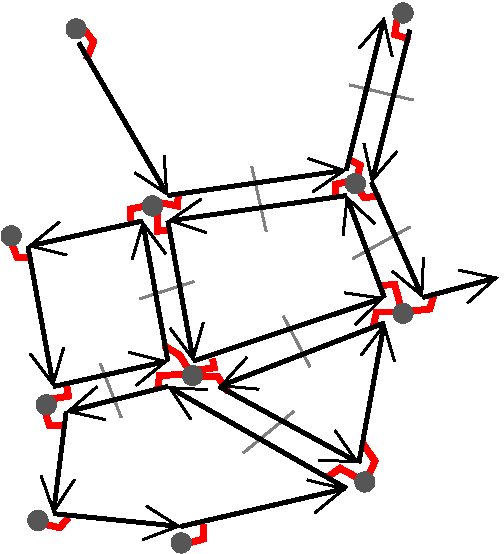
\includegraphics[width=.25\textwidth]
    {Linear_cell_complex/fig/pdf/plane-graph}
  \qquad
  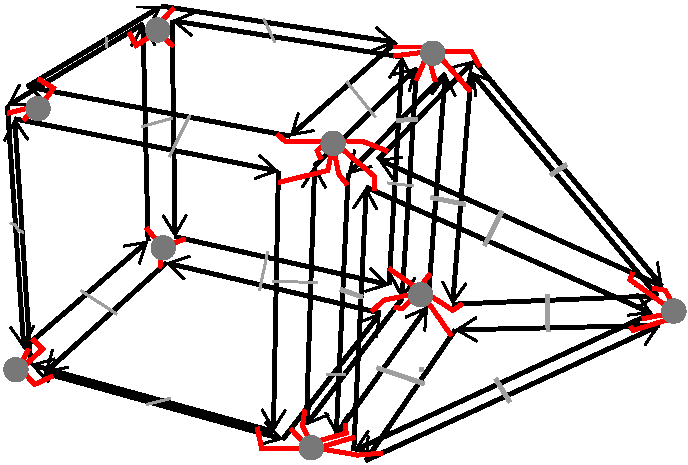
\includegraphics[width=.45\textwidth]
  {Linear_cell_complex/fig/pdf/basic-example3D}}
\end{ccTexOnly}
\begin{ccHtmlOnly}
  <CENTER>
  <A HREF="fig/png/plane-graph.png">
      <img src="fig/png/plane-graph.png" alt=""></A>
  <A HREF="fig/png/basic-example3D.png">
      <img src="fig/png/basic-example3D.png" alt=""></A>
  </CENTER>
\end{ccHtmlOnly}
\caption{Examples of \ccc{CGAL::Linear_cell_complex}. Gray disks show the
  attributes associated to vertices. Associations between darts and
  attributes are drawn by small lines between darts and disks.
  \textbf{Left:}~Example of \ccc{CGAL::Linear_cell_complex<2,2>}.
  \textbf{Right:}~Example of \ccc{CGAL::Linear_cell_complex<3,3>}.}
\label{fig-combi_map_with_point}
\end{figure}

\subsection{Cell Attributes}\label{ssec-attribute-wp}

The
\ccc{CGAL::Cell_attribute_with_point<LCC,Info_,Tag,OnMerge,OnSplit>}
class is a model of the \ccc{CellAttributeWithPoint} concept, which is
a refinement of the \ccc{CellAttribute} concept. It represents an
attribute associated with a cell, which can contain an information
(depending on whether \ccc{Info_==void} or not), but which always
contains a point, an instance of \ccc{LCC::Point}.

\subsection{Linear Cell Complex Traits}\label{ssec-lcc-traits}

The \ccc{LinearCellComplexTraits} geometric traits concept defines the
required types and functors used in the \ccc{Linear_cell_complex}
class. For example it defines \ccc{Point}, the type of points used,
and \ccc{Vector}, the corresponding vector type.  It also defines all
the required functors used for constructions and operations, as for
example \ccc{Construct_translated_point} or
\ccc{Construct_sum_of_vectors}.

The class \ccc{CGAL::Linear_cell_complex_traits<d,K>} is a model of
\ccc{LinearCellComplexTraits}. It defines the different types which
are obtained from \ccc{K} that, depending on \ccc{d}, is a model of
the concept \ccc{Kernel} if \ccc{d==2} or \ccc{d==3}, and a model of
the concept \ccc{Kernel_d} otherwise.


\subsection{Linear Cell Complex Items}\label{ssec-lcc-item}

The \ccc{LinearCellComplexItems} concept refines the
\ccc{CombinatorialMapItems} concept by adding the requirement that
0-attributes are enabled, and associated with a type of attribute
being a model of the \ccc{CellAttributeWithPoint} concept.  

The class \ccc{CGAL::Linear_cell_complex_min_items<d>} is a
model of \ccc{LinearCellComplexItems}. It uses \ccc{CGAL::Dart<d>},
and instances of \ccc{CGAL::Cell_attribute_with_point}
(which contain no information) associated to each vertex. All other
attributes are void.  

\section{Operations}

Several operations defined in the combinatorial maps package can be
used on a linear cell complex. This is the case for all the iteration
operations that do not modify the model (see example in 
Section~\ref{ssec-3D-lcc}). This is also the case for
all the operations that do not create new 0-cells: \ccc{sew},
\ccc{unsew}, \ccc{remove_cell}, \ccc{insert_cell_1_in_cell_2},
\ccc{insert_cell_2_in_cell_3}.  Indeed, all these operations update
non void attributes, and thus update vertex attributes of a linear
cell complex. Note that some existing 0-attributes can be duplicated
by the \ccc{unsew} method, but these 0-attributes are not new but
copies of existing old 0-attributes.

However, operations that create a new 0-cell can not be directly used
since the new 0-cell would not be associated with a vertex
attribute. Indeed, it is not possible for these operations to
automatically decide which point to create. These operations are:
\ccc{insert_cell_0_in_cell_1}, \ccc{insert_cell_0_in_cell_2}
\ccc{insert_dangling_cell_1_in_cell_2}, plus all the creation
operations. For these operations, new versions are proposed taking
some points as additional parameters.  Lastly, some new operations are
defined, which use the geometry (see sections~\ref{ssec-constructions-op} and
\ref{ssec-modif-op}).

All the operations given in this section guarantee that given a valid
linear cell complex and a possible operation, the result is a valid
linear cell complex. As for a combinatorial map, it is also possible
to use low level operations but additional operations may be needed to
restore the validity conditions.

\subsection{Sewing and Unsewing \label{ssec-lcc-link-darts}}

As explained in the combinatorial map user manual,
Section~\ref{ssec-link-darts}, it is possible to glue two \emph{i}-cells
along an (\emph{i}-1)-cell by using the \ccc{sew<i>} method. Since
this method updates non void attributes, and since points are specific
attributes, they are automatically updated during the \ccc{sew<i>}
method. Thus the sewing of two \emph{i}-cells could deform the
geometry of the concerned objects.

For example, in Figure~\ref{fig-lcc-exemple-sew}, we want to 3-sew the
two initial 3-cells. \ccc{sew<3>(1,5)} links by \betatrois{} the pairs
of darts (1,5), (2,8), (3,7) and (4,6). The eight vertex attributes
around the facet between the two 3-cells before the sew are merged by
pair during the sew operation (and the \ccc{On_merge} functor is
called four times). Thus, after the sew, there are only four
0-attributes around the facet. By default, the attributes associated
with the first dart of the sew operation are kept (but this can be
modified by defining your own functor in the attribute class as
explained in the package combinatorial map, Section~\ref{ssec-link-darts}). 
Intuitively, the
geometry of the second 2-cell is deformed to fit to the first 2-cell.
%
\def\LargFig{.45\textwidth}
\begin{figure}
  \begin{ccTexOnly}
    \begin{center}
      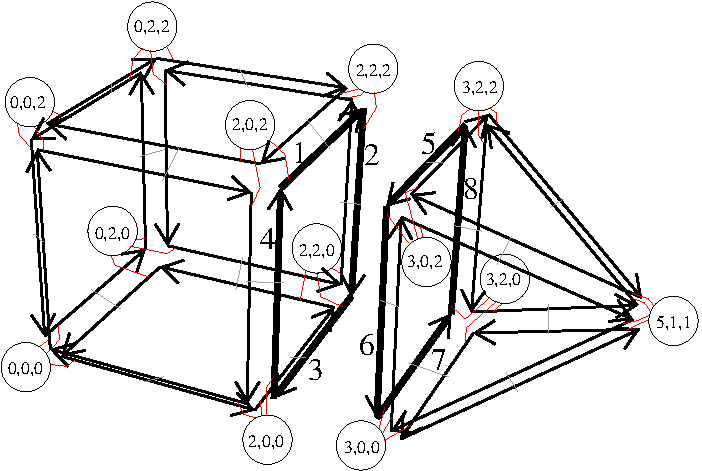
\includegraphics[width=\LargFig]{Linear_cell_complex/fig/pdf/exemple-carte-with_point_3d-sew}\qquad
      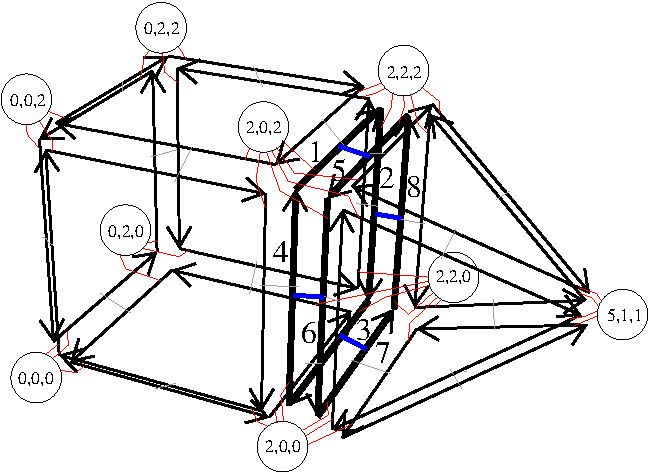
\includegraphics[width=\LargFig]{Linear_cell_complex/fig/pdf/exemple-carte-with_point_3d-sew2}
    \end{center}
  \end{ccTexOnly}
  \begin{ccHtmlOnly}
    <CENTER>
    <A HREF="fig/png/exemple-carte-with_point_3d-sew.png">
        <img src="fig/png/exemple-carte-with_point_3d-sew.png" alt=""></A>
    <A HREF="fig/png/exemple-carte-with_point_3d-sew2.png">
        <img src="fig/png/exemple-carte-with_point_3d-sew2.png" alt=""></A>
    </CENTER>
    \end{ccHtmlOnly}
    \caption{Example of 3-sew operation for linear cell complex.
      \textbf{Left}: A 3D linear cell complex containing two 3-cells
      that are not connected. Vertex attributes are drawn with circles
      containing point coordinates.  Associations between darts and
      attributes are drawn with small lines between darts and
      disks. \textbf{Right}: The 3D linear cell complex obtained as
      result of \ccc{sew<3>(1,5)} (or \ccc{sew<3>(2,8)}, or
      \ccc{sew<3>(3,7)}, or \ccc{sew<3>(4,6)}).  The eight
      0-attributes around the facet between the two 3-cells before the
      sew operation, are merged into four 0-attributes after. The
      geometry of the pyramid is deformed since its base is fitted on
      the 2-cell of the cube.}
    \label{fig-lcc-exemple-sew}
\end{figure} 

This is similar for the unsew operation, which removes \betai{} links
of all the darts in
\orbit{\betaun{},\myldots{},\betaimdeux{},\betaipdeux{},\myldots{},\betad{}}(\emph{d0}), 
and updates
non void attributes which are no more associated to a same cell due to
the unlinks.  If we take the linear cell complex given in
Figure~\ref{fig-lcc-exemple-sew} (Right), and we call
\ccc{unsew<3>(2)}, we obtain the linear cell complex in
Figure~\ref{fig-lcc-exemple-sew} (Left) except for the coordinates of
the new four vertices, which by default are copies of original
vertices (this behavior can be modified thanks to the functor
\ccc{On_split} in the attribute class).  The \ccc{unsew<3>} operation
has removed the four \betatrois{} links, and has duplicated the 0-attributes
since vertices are split in two after the unsew operation.

\subsection{Construction Operations}\label{ssec-constructions-op}

There are several member functions allowing to insert specific
configurations of darts into a linear cell complex. These functions
return a \ccc{Dart_handle} to the new object.  Note
that the dimension of the linear cell complex must be large enough:
darts must contain all the \betats{} used by the operation.  All these
methods add new darts in the current linear cell complex, existing
darts are not modified. These functions
are \ccc{make_segment}, \ccc{make_triangle}, 
\ccc{make_tetrahedron} and \ccc{make_hexahedron}. 

There are two functions allowing to build a linear cell complex
from two other \cgal\ data types:
\begin{itemize}
\item \ccc{import_from_triangulation_3(lcc,atr)}: adds in \ccc{lcc} all 
  the tetrahedra present in \ccc{atr}, a \ccc{CGAL::Triangulation_3};
\item \ccc{import_from_polyhedron_3(lcc,ap)}: adds in \ccc{lcc} all 
  the cells present in \ccc{ap}, a \ccc{CGAL::Polyhedron_3}.
\end{itemize}

Lastly, the function \ccc{import_from_plane_graph(lcc,ais)} adds in
\ccc{lcc} all the cells reconstructed from the planar graph read in
\ccc{ais}, a \ccc{std::istream} (see the reference manual for the file
format).

\subsection{Modification Operations}\label{ssec-modif-op}

Some methods are defined in \ccc{Linear_cell_complex} class
to modify a linear cell complex and update the vertex attributes.  In
the following, we denote by \ccc{dh0}, \ccc{dh1}, \ccc{dh2} the dart
handles for the darts \ccc{d0}, \ccc{d1}, \ccc{d2}, respectively. That
is \ccc{d0 == *dh0}.

%%%%%%%%%%%%%%%%%%%%%%%%%%%%%%%%%%%%%%%%%%%%%%%%%%%%%%%%%%%%%%%%%%%%%%%%%%%%%%
\begin{figure}[htb]
  \begin{ccTexOnly}
    \begin{center}
      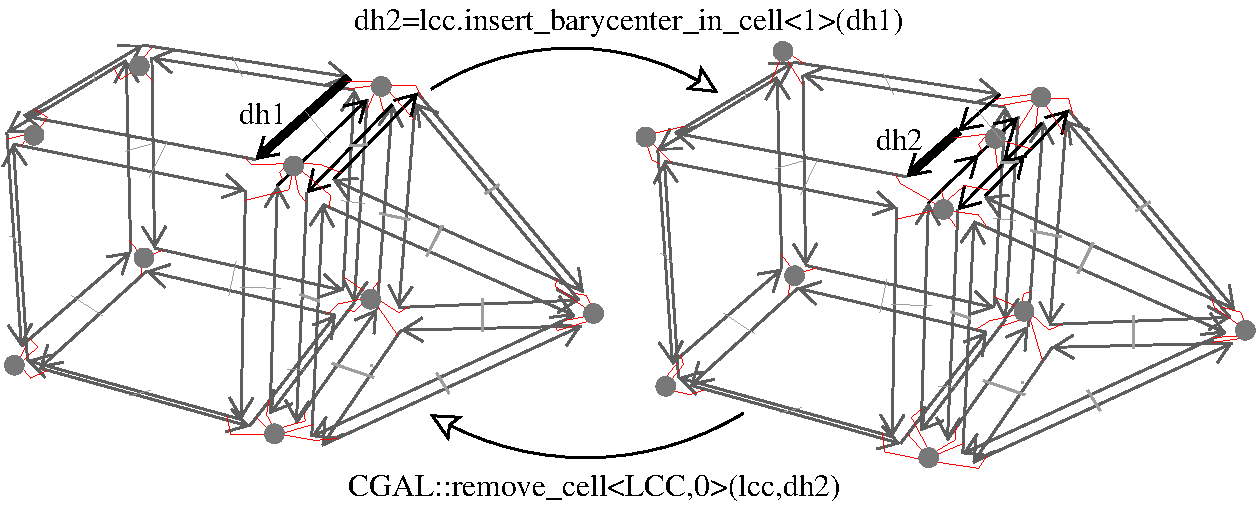
\includegraphics[width=.75\textwidth]{Linear_cell_complex/fig/pdf/insert-vertex}
    \end{center}
  \end{ccTexOnly}
  \begin{ccHtmlOnly}
    <CENTER> <A HREF="fig/png/insert-vertex.png"><img
    src="fig/png/insert-vertex.png" alt=""></A> </CENTER>
  \end{ccHtmlOnly}
  \caption{Example of \ccc{insert_barycenter_in_cell<1>} and
    \ccc{remove_cell<0>} operations. \textbf{Left}: Initial linear
    cell complex.  \textbf{Right}: After the insertion of a point in
    the barycenter of the 1-cell containing dart \emph{d1}.  Now if we
    remove the 0-cell containing dart \emph{d2}, we obtain a linear
    cell complex isomorphic to the initial one.}
  \label{fig-lcc-insert-vertex}
\end{figure}
%%%%%%%%%%%%%%%%%%%%%%%%%%%%%%%%%%%%%%%%%%%%%%%%%%%%%%%%%%%%%%%%%%%%%%%%%%%%%%

\ccc{lcc.insert_barycenter_in_cell<unsigned int i>(dh0)} adds the
barycenter of the \emph{i}-cell containing dart \ccc{d0}. This
operation is possible if \ccc{d0}\myin{}\ccc{lcc.darts()} (see examples
on Figure~\ref{fig-lcc-insert-vertex} and
Figure~\ref{fig-lcc-triangulate}).

\ccc{lcc.insert_point_in_cell<unsigned int i>(dh0,p)} is an operation
similar to the previous operation, the only difference being that the
coordinates of the new point are here given by \ccc{p} instead of being
computed as the barycenter of the \emph{i}-cell.  Currently, these two
operations are only defined for \ccc{i=1} to insert a point in an
edge, or \ccc{i=2} to insert a point in a facet.
\begin{figure}[htb]
  \begin{ccTexOnly}
    \centerline{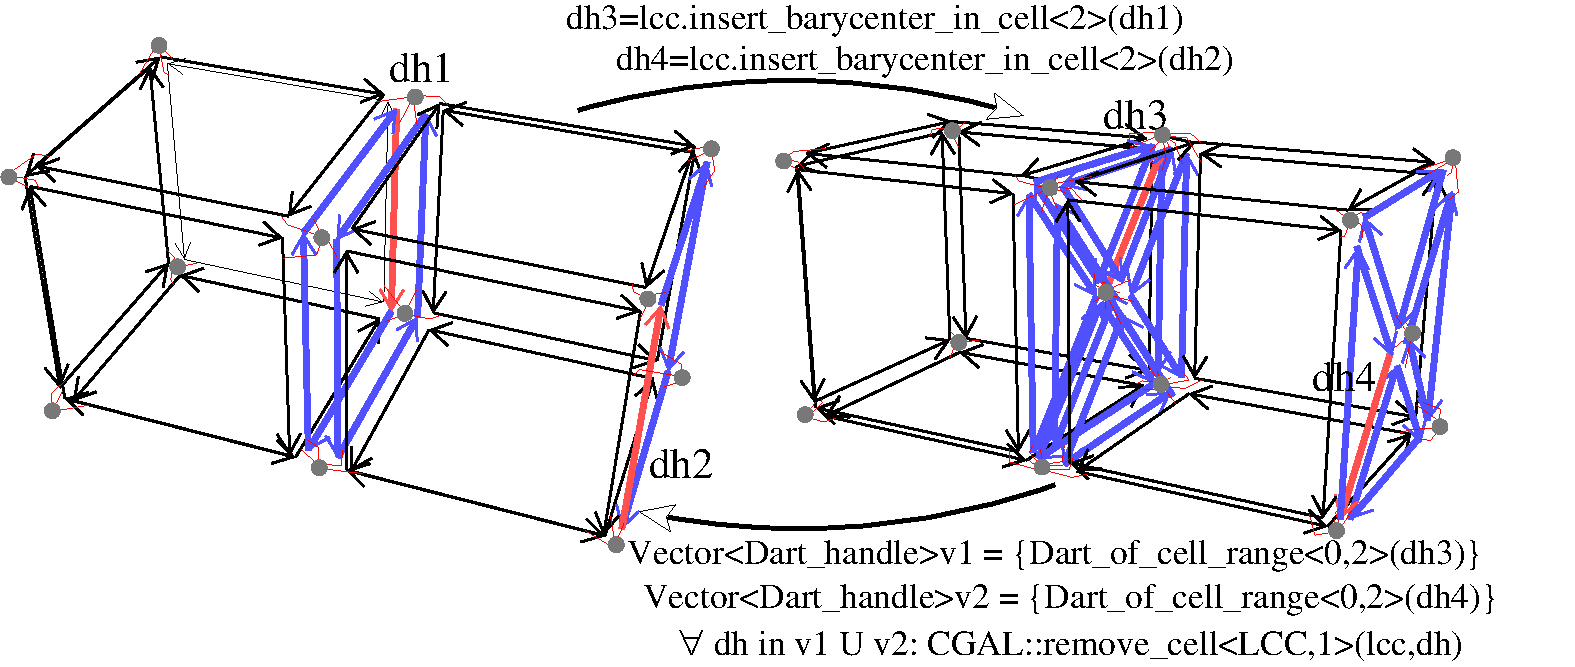
\includegraphics[width=.85\textwidth]
      {Linear_cell_complex/fig/pdf/triangulation}}
  \end{ccTexOnly}
  \begin{ccHtmlOnly}
    <CENTER> <A HREF="fig/png/triangulation.png"> <img
    src="fig/png/triangulation.png" alt=""></A> </CENTER>
  \end{ccHtmlOnly}
  \caption{Examples of \ccc{insert_barycenter_in_cell<2>} operation.}
  \label{fig-lcc-triangulate}
\end{figure}
%

\ccc{lcc.insert_dangling_cell_1_in_cell_2(dh0,p)} adds a 1-cell in
the 2-cell containing dart \ccc{d0}, the 1-cell being attached by only
one of its vertex to the 0-cell containing dart \ccc{d0}.  The second
vertex of the new edge is associated with a new 0-attribute containing
a copy of \ccc{p} as point. This operation is possible if
\ccc{d0}\myin{}\ccc{lcc.darts()} (see example on
Figure~\ref{fig-lcc-insert-dangling-edge}).
  \begin{figure}[htb]
    \begin{ccTexOnly}
      \begin{center}
        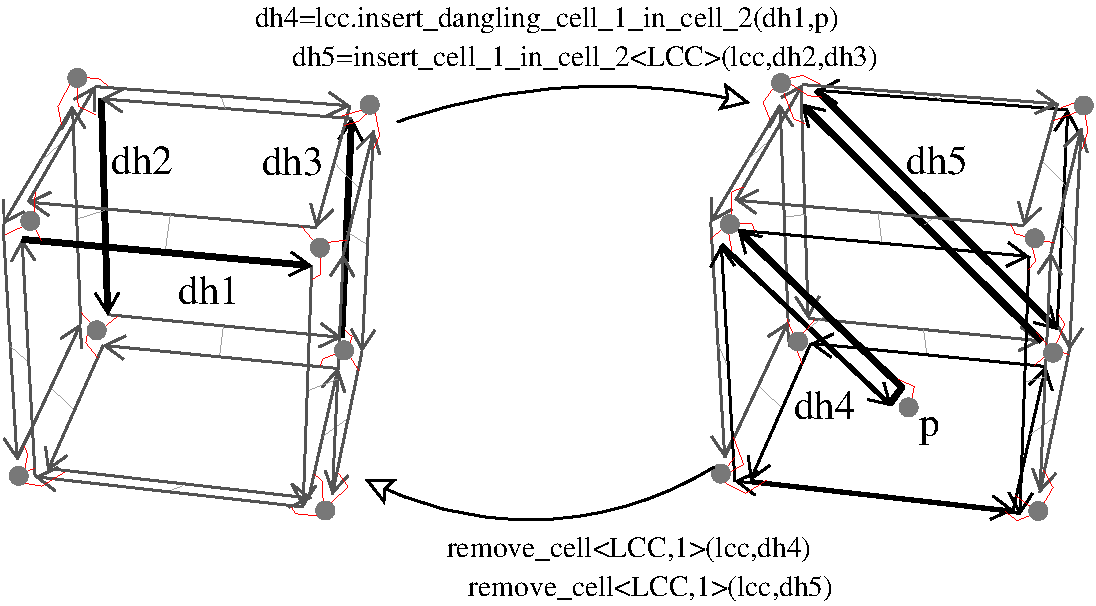
\includegraphics[width=.72\textwidth]{Linear_cell_complex/fig/pdf/insert-edge}
      \end{center}
    \end{ccTexOnly}
    \begin{ccHtmlOnly}
      <CENTER> <A HREF="fig/png/insert-edge.png"><img
      src="fig/png/insert-edge.png" alt=""></A> </CENTER>
    \end{ccHtmlOnly}
    \caption{Example of \ccc{insert_dangling_cell_1_in_cell_2},
      \ccc{insert_cell_1_in_cell_2} and
      \ccc{remove_cell<1>} operations. \textbf{Left}: Initial linear
      cell complex.  \textbf{Right}: After the insertion of a dangling
      1-cell in the 2-cell containing dart \emph{d1}, and of a 1-cell
      in the 2-cell containing dart \emph{d2}. Now if we remove
      the 1-cells containing dart \emph{d4} and \emph{d5},
      we obtain a linear cell complex isomorphic to the initial one.}
    \label{fig-lcc-insert-dangling-edge}
  \end{figure}

  Some examples of use of these operations are given in
  Section~\ref{ssec-5dexample}.

\section{Examples}

\subsection{A 3D Linear Cell Complex}\label{ssec-3D-lcc}

This example uses a 3-dimensional linear cell complex. It creates two
tetrahedra and displays all the points of the linear cell complex
thanks to a \ccc{Vertex_attribute_const_range}. Then, the two
tetrahedra are 3-sewn and we translate all the points of the second
tetrahedron along vector \ccc{v(3,1,1)}.  Since the two tetrahedra
are 3-sewn, this translation moves also the 2-cell of the first
tetrahedron shared with the second one.  This is illustrated by
displaying all the points of each 3-cell. For that we use a
\ccc{std::for_each} and the \ccc{Display_vol_vertices} functor.

\ccIncludeExampleCode{Linear_cell_complex/linear_cell_complex_3.cpp}

The output is:
\begin{verbatim}
Vertices: 1 1 2; 1 0 0; 0 2 0; -1 0 0; 1 1 -3; 1 0 -1; -1 0 -1; 0 2 -1; 
Volume 1 : -1 0 0; 0 2 0; 1 0 0; 1 1 2; 
Volume 2 : 0 2 -1; -1 0 -1; 1 0 -1; 1 1 -3; 
Volume 1 : -1 0 0; 0 2 0; 1 0 0; 1 1 2; 
Volume 2 : 0 2 0; -1 0 0; 1 0 0; 1 1 -3; 
Volume 1 : 2 1 1; 3 3 1; 4 1 1; 1 1 2; 
Volume 2 : 3 3 1; 2 1 1; 4 1 1; 4 2 -2; 
LCC characteristics: #Darts=24, #0-cells=5, #1-cells=9, #2-cells=7, #3-cells=2, #ccs=1, valid=1
\end{verbatim}

The first line gives the points of the linear cell complex before the
\ccc{sew<3>}. There are eight points, four for each tetrahedron.
After the sew, six vertices are merged two by two, thus there are five
vertices. We can see the points of each 3-cell (lines Volume 1 and
Volume 2) before the sew, after the sew and after the translation of
the second volume.  We can see that this translation has also modified
the three common points between the two 3-cells.  The last line shows
the number of cells of the linear cell complex, the number of
connected components, and finally a Boolean to show the validity of
the linear cell complex.

\subsection{A 4D Linear Cell Complex}\label{ssec-5dexample}

This example uses a 4-dimensional linear cell complex embedded in a
5-dimensional ambient space.  It creates two tetrahedra having 5D
points and sews the two tetrahedra by \betaquatre{}. Then we use some high
level operations, display the number of cells of the linear cell
complex, and check its validity.  Last we use the reverse operations
to get back to the initial configuration.

\ccIncludeExampleCode{Linear_cell_complex/linear_cell_complex_4.cpp}

The output is:
\begin{verbatim}
#Darts=24, #0-cells=8, #1-cells=12, #2-cells=8, #3-cells=2, #4-cells=2, #ccs=2, valid=1
#Darts=24, #0-cells=4, #1-cells=6, #2-cells=4, #3-cells=1, #4-cells=2, #ccs=1, valid=1
#Darts=28, #0-cells=5, #1-cells=7, #2-cells=4, #3-cells=1, #4-cells=2, #ccs=1, valid=1
#Darts=32, #0-cells=5, #1-cells=8, #2-cells=5, #3-cells=1, #4-cells=2, #ccs=1, valid=1
#Darts=24, #0-cells=8, #1-cells=12, #2-cells=8, #3-cells=2, #4-cells=2, #ccs=2, valid=1
\end{verbatim}

\subsection{A 3D Linear Cell Complex with Colored Vertices}
\label{ssec-exemple-color-vertices}

This example illustrates the way to use a 3D linear cell complex by
adding another information to vertices. For that, we need to define
our own items class.  The difference with the
\ccc{CGAL::Linear_cell_complex_min_items} class is about the definition of
the vertex attribute where we use a \ccc{CGAL::Cell_attribute_with_point}
with a non void info. In this example, the "vextex color" is just
given by an \ccc{int} (the second template parameter of the
\ccc{CGAL::Cell_attribute_with_point}).  Lastly, we define the
\ccc{Average_functor} class in order to set the color of a vertex
resulting of the merging of two vertices to the average of the two
initial values. This functor is associated with the vertex attribute
by passing it as template parameter.  Using this items class instead of
the default one is done during the instantiation of template
parameters of the \ccc{CGAL::Linear_cell_complex} class.

Now we can use \ccc{LCC_3} in which each vertex is associated with an
attribute containing both a point and an information. In the following
example, we create two cubes, and set the color of the vertices of the
first cube to 1 and of the second cube to 19 (by iterating through two
\ccc{One_dart_per_incident_cell_range<0, 3>} ranges).  Then we
\emph{3-sew} the two cubes along one facet. This operation merges some
vertices (as in the example of Figure~\ref{fig-lcc-exemple-sew}).  We
insert a vertex in the common 2-cell between the two cubes, and set
the information of the new 0-attribute to 5.  In the last loop, we
display the point and the information of each vertex of the linear
cell complex.

\ccIncludeExampleCode{Linear_cell_complex/linear_cell_complex_3_with_colored_vertices.cpp}

The output is:
\begin{verbatim}
point: -1 1 1, color: 10
point: -1 0 1, color: 10
point: -2 0 1, color: 1
point: -2 1 1, color: 1
point: -2 1 0, color: 1
point: -1 1 0, color: 10
point: -1 0 0, color: 10
point: -2 0 0, color: 1
point: 1 1 1, color: 19
point: 1 0 1, color: 19
point: -1 0.5 0.5, color: 5
point: 1 1 0, color: 19
point: 1 0 0, color: 19
\end{verbatim}

Before applying the sew operation, the eight vertices of the first
cube are colored by 1, and the eight vertices of the second cube by
19. After the sew operation, there are eight vertices which are merged
two by two, and due to the average functor, the color of the four
resulting vertices is now 10. Then we insert a vertex in the center
of the common 2-cell between the two cubes.  The coordinates of this
vertex are initialized with the barycenter of the 2-cell
(-1,0.5,0.5), and its color is not initialized by the method, thus we
set its color manually by using the result of
\ccc{insert_barycenter_in_cell<2>} which is a dart incident to the
new vertex.

\section{Design and Implementation History}

This package was developed by Guillaume Damiand, with the help of
Andreas Fabri, S\'ebastien Loriot and Laurent Rineau.  Monique
Teillaud and Bernd G{\"a}rtner contributed to the manual.
